\documentclass[]{article}

\usepackage{graphicx, wrapfig}
\usepackage{float}
%opening
\title{Theft Tracker: A Localization Algorithm to Track Position of Stolen Vehicles using WSN}
\author{Giorgio Cozza (CP:10649461, MAT:904965)}

\begin{document}

\maketitle

\section{Problem}

GPS is one of the most popular technology for object localization around the earth, usually employeed by car antitheft systems to localize stolen vehicles. Unfortunately in most of the cases such kind of service is subjected to a fee that customers do not consider convenient especially for vehicles without the sufficient technology to support it. 
Theft Tracker tries to overcome this limitation by using sensor nodes located on vehicles to broadcast alert messages to the neighbour nodes in case the car gets stolen and the traffic is then broadcasted by the receivers until a \textbf{network gateway} is reached. Such type of mote provided with GPS uses a rough estimation of the distance from the origin that sends together with its coordinates to the server.


\section{Solution}

\begin{wrapfigure}{r}{5.5cm}
\vspace{-50pt}
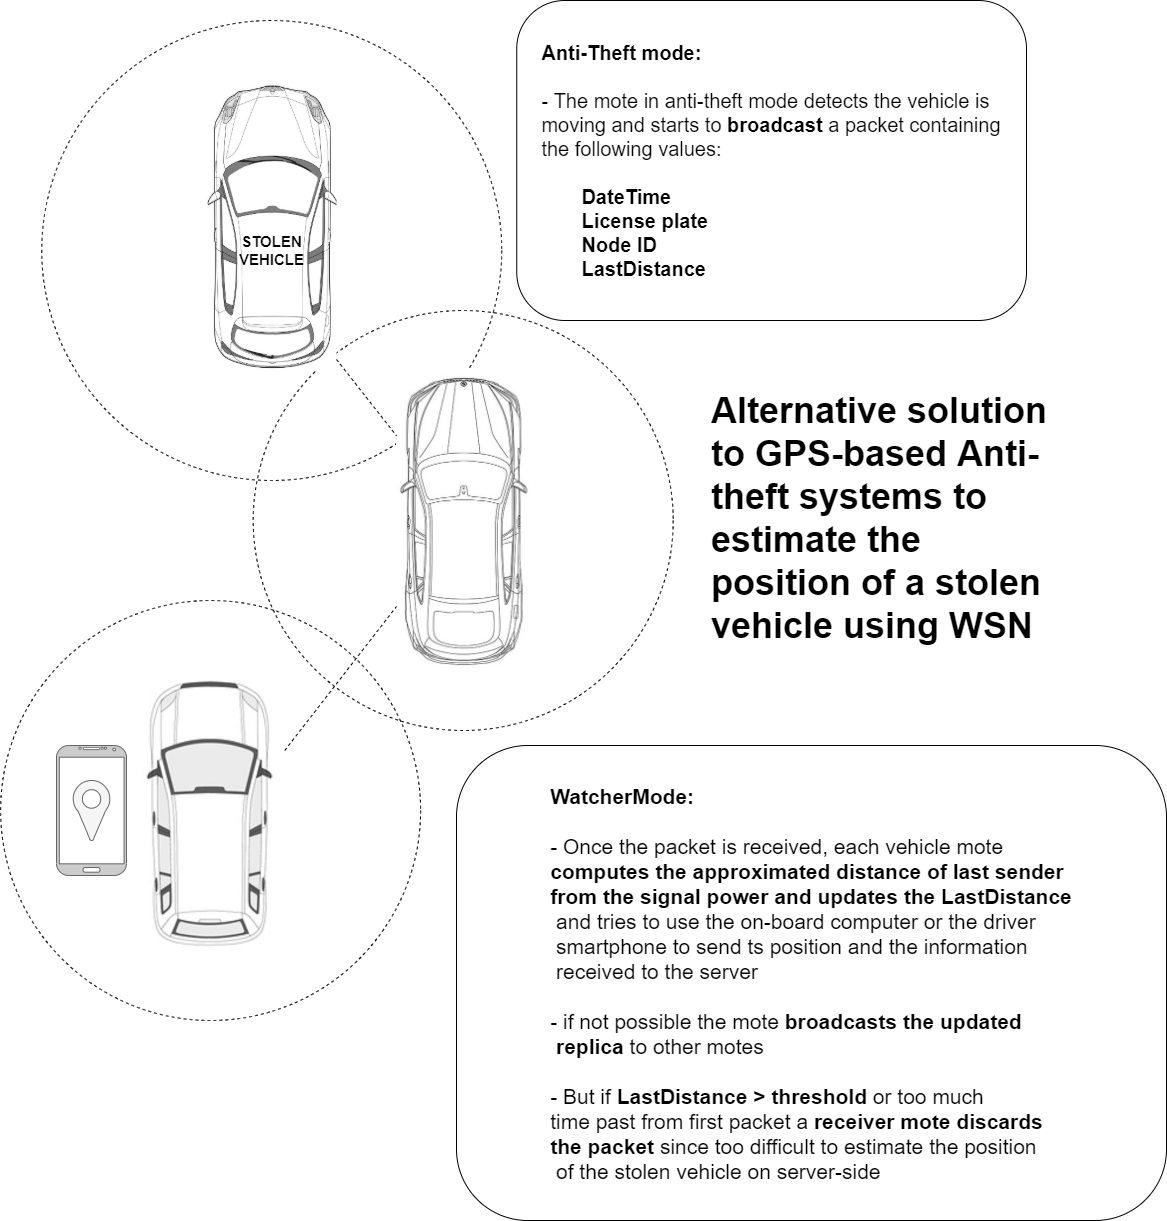
\includegraphics[width=7.5cm]{./images/theft_tracker_summary.png}
\caption{Theft Tracker summary.}\label{tt-fig:1}
\vspace{-70pt}
\end{wrapfigure}

\subsection{Mote Application}

The application conceived for constrained sensor nodes runs on Contiki OS. Two different programs are developed, one for the simple mote in charge of broadcasting alert messages received from the stolen vehicle or from other motes (\textbf{ttmote}) and one for the network gateway (\textbf{ttgateway}) that sends the GPS coordinates together with a distance estimation from the origin to the server. The information exchanged by the ttmotes includes:
\begin{itemize}
	\item \textbf{first mote ID}: an identification number of the alert origin
\end{itemize}
\newpage
\begin{itemize}
	\item \textbf{event clock time}: the number of seconds elapsed from the moment the mote switched on to the theft event 
	\item \textbf{origin clock time}: the number of seconds elapsed from the moment the mote switched on to the send of the first alert message from the origin (stolen vehicle) 
	\item\textbf{hop count}: the number of motes an alert message traversed
	\item \textbf{last distance}: the estimation of the distance computed so far from the origin exploiting the RSSI of each mote from the last hop.
	\item \textbf{hop list}: the list of motes that an alert message traversed at each step used to avoid closed loops
	\item \textbf{vehicle identification number}: according to the ISO 3779 a unique identifier of the vehicle
\end{itemize}
In both the ttmote and ttgateway two protothreads run simultaneously:
\begin{itemize}
	\item the \textbf{guard}: that is in charge of detecting events that change the status of the mote (e.g: the vehicle is stolen)
	\item the \textbf{shouter}: that broadcasts all the received alerts to the neighbour nodes or forges new alert messages if the vehicle is stolen.
\end{itemize}
The theft detection can be performed in different ways but since such part of the system requires a proper emulation of some feature of the mote in Cooja (e.g: accelerometer) which is not provided, the condition that notifies the event is triggered using the mote button.\par 
The mote application keeps track of the alerts exchanged by the motes in an \textbf{alert session} data structure, that is initialized when a \textbf{new acceptable} alert message is received by a node, it makes use of two timers, the \textbf{send timer} that triggers each second an alert message and a \textbf{session timer}, that expires in 30 seconds, the interval in which a received alert is broadcasted to all the neighbour nodes. But the mote application does not relay all the alerts received. In order to start a new alert session or restart the session timer, an alert must be:
\begin{itemize}
	\item \textbf{new}: it includes a smaller estimation of the distance from the stolen vehicle 
	\item \textbf{acceptable}: the estimated distance from the origin, or the time elapsed from the origin clock time are not too large (e.g: acceptable distance: 200 [m], acceptable interval: 30 [s]) and alerts are not exchanged in a closed loop
\end{itemize}
In order to implement the hop list, the related operations and some other function, a static library is generated and included in the binary file at compile-time. \par 
The mote and gateway applications moreover are realized for a Sky mote, unprovided with a GPS module. For such reason, in the gateway application fake coordinates are hard-coded in the source files simulating a static device sending the alert to the server. 

\subsection{Server Application}
The server-side application is implemented using Node-RED. A single flow includes as many TCP sockets as active gateways, in this case there is a simple application able to manage a single alert session. Since the gateway mote streams data in form of text lines (i.e: key: value) the \textbf{message processing} node keeps track of the information related to a single alert in the flow context and once completely received sends the message to the \textbf{alert scheduler}.\par Since motes replicates and broadcast alerts even when the origin node gets out of range for a certain time interval (i.e: acceptable time interval), it may happen that a gateway continues to receive and sends messages to the Internet when simultaneously the origin mote approaches another gateway, the backend server in such case captures two messages from two different gateways providing a bouncing position in the map. The scheduler simply discards the messages from the previous gateway by checking the origin clock time.\par
Finally the \textbf{worldmap message format} prepares each alert in order to be interpreted and displayed by the \textbf{worldmap} node in the map.

\begin{figure}[h!]
	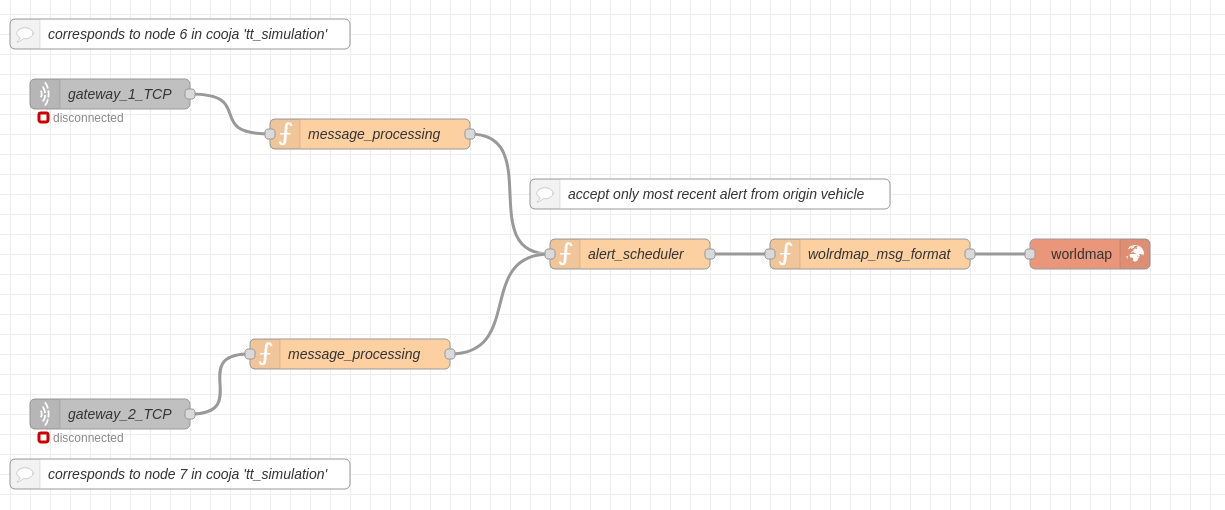
\includegraphics[scale=0.3]{./images/tt_server_arc.png}
	\caption{Server on Node-RED flow.}\label{tt-fig:2}
\end{figure}

\subsection{Cooja Simulation}
In
\end{document}
